\documentclass[12pt]{beamer}\usepackage[]{graphicx}\usepackage[]{color}
%% maxwidth is the original width if it is less than linewidth
%% otherwise use linewidth (to make sure the graphics do not exceed the margin)
\makeatletter
\def\maxwidth{ %
  \ifdim\Gin@nat@width>\linewidth
    \linewidth
  \else
    \Gin@nat@width
  \fi
}
\makeatother

\definecolor{fgcolor}{rgb}{0.345, 0.345, 0.345}
\newcommand{\hlnum}[1]{\textcolor[rgb]{0.686,0.059,0.569}{#1}}%
\newcommand{\hlstr}[1]{\textcolor[rgb]{0.192,0.494,0.8}{#1}}%
\newcommand{\hlcom}[1]{\textcolor[rgb]{0.678,0.584,0.686}{\textit{#1}}}%
\newcommand{\hlopt}[1]{\textcolor[rgb]{0,0,0}{#1}}%
\newcommand{\hlstd}[1]{\textcolor[rgb]{0.345,0.345,0.345}{#1}}%
\newcommand{\hlkwa}[1]{\textcolor[rgb]{0.161,0.373,0.58}{\textbf{#1}}}%
\newcommand{\hlkwb}[1]{\textcolor[rgb]{0.69,0.353,0.396}{#1}}%
\newcommand{\hlkwc}[1]{\textcolor[rgb]{0.333,0.667,0.333}{#1}}%
\newcommand{\hlkwd}[1]{\textcolor[rgb]{0.737,0.353,0.396}{\textbf{#1}}}%

\usepackage{framed}
\makeatletter
\newenvironment{kframe}{%
 \def\at@end@of@kframe{}%
 \ifinner\ifhmode%
  \def\at@end@of@kframe{\end{minipage}}%
  \begin{minipage}{\columnwidth}%
 \fi\fi%
 \def\FrameCommand##1{\hskip\@totalleftmargin \hskip-\fboxsep
 \colorbox{shadecolor}{##1}\hskip-\fboxsep
     % There is no \\@totalrightmargin, so:
     \hskip-\linewidth \hskip-\@totalleftmargin \hskip\columnwidth}%
 \MakeFramed {\advance\hsize-\width
   \@totalleftmargin\z@ \linewidth\hsize
   \@setminipage}}%
 {\par\unskip\endMakeFramed%
 \at@end@of@kframe}
\makeatother

\definecolor{shadecolor}{rgb}{.97, .97, .97}
\definecolor{messagecolor}{rgb}{0, 0, 0}
\definecolor{warningcolor}{rgb}{1, 0, 1}
\definecolor{errorcolor}{rgb}{1, 0, 0}
\newenvironment{knitrout}{}{} % an empty environment to be redefined in TeX

\usepackage{alltt}
\usepackage{graphicx}
\usepackage{tikz}
\setbeameroption{hide notes}
\setbeamertemplate{note page}[plain]
\usepackage{listings}

% get rid of junk
\usetheme{default}
\usefonttheme[onlymath]{serif}
\beamertemplatenavigationsymbolsempty
\hypersetup{pdfpagemode=UseNone} % don't show bookmarks on initial view

% named colors
\definecolor{offwhite}{RGB}{255,250,240}
\definecolor{gray}{RGB}{155,155,155}

\ifx\notescolors\undefined % slides

  \definecolor{foreground}{RGB}{80,80,80}
  \definecolor{background}{RGB}{255,255,255}
  \definecolor{title}{RGB}{255,199,0}
  \definecolor{subtitle}{RGB}{89,132,212}
  \definecolor{hilit}{RGB}{248,117,79}
  \definecolor{vhilit}{RGB}{255,111,207}
  \definecolor{lolit}{RGB}{200,200,200}
  \definecolor{lit}{RGB}{255,199,0}
  \definecolor{mdlit}{RGB}{89,132,212}
  \definecolor{link}{RGB}{248,117,79}

\else % notes
  \definecolor{background}{RGB}{255,255,255}
  \definecolor{foreground}{RGB}{24,24,24}
  \definecolor{title}{RGB}{27,94,134}
  \definecolor{subtitle}{RGB}{22,175,124}
  \definecolor{hilit}{RGB}{122,0,128}
  \definecolor{vhilit}{RGB}{255,0,128}
  \definecolor{lolit}{RGB}{95,95,95}
\fi
\definecolor{nhilit}{RGB}{128,0,128}  % hilit color in notes
\definecolor{nvhilit}{RGB}{255,0,128} % vhilit for notes

\newcommand{\hilit}{\color{hilit}}
\newcommand{\vhilit}{\color{vhilit}}
\newcommand{\nhilit}{\color{nhilit}}
\newcommand{\nvhilit}{\color{nvhilit}}
\newcommand{\lit}{\color{lit}}
\newcommand{\mdlit}{\color{mdlit}}
\newcommand{\lolit}{\color{lolit}}

% use those colors
\setbeamercolor{titlelike}{fg=title}
\setbeamercolor{subtitle}{fg=subtitle}
\setbeamercolor{frametitle}{fg=gray}
\setbeamercolor{structure}{fg=subtitle}
\setbeamercolor{institute}{fg=lolit}
\setbeamercolor{normal text}{fg=foreground,bg=background}
%\setbeamercolor{item}{fg=foreground} % color of bullets
%\setbeamercolor{subitem}{fg=hilit}
%\setbeamercolor{itemize/enumerate subbody}{fg=lolit}
\setbeamertemplate{itemize subitem}{{\textendash}}
\setbeamerfont{itemize/enumerate subbody}{size=\footnotesize}
\setbeamerfont{itemize/enumerate subitem}{size=\footnotesize}

% center title of slides
\setbeamertemplate{blocks}[rounded]
\setbeamertemplate{frametitle}[default][center]
% margins
\setbeamersize{text margin left=25pt,text margin right=25pt}

% page number
\setbeamertemplate{footline}{%
    \raisebox{5pt}{\makebox[\paperwidth]{\hfill\makebox[20pt]{\lolit
          \scriptsize\insertframenumber}}}\hspace*{5pt}}

% add a bit of space at the top of the notes page
\addtobeamertemplate{note page}{\setlength{\parskip}{12pt}}

% default link color
\hypersetup{colorlinks, urlcolor={link}}

\ifx\notescolors\undefined % slides
  % set up listing environment
  \lstset{language=bash,
          basicstyle=\ttfamily\scriptsize,
          frame=single,
          commentstyle=,
          backgroundcolor=\color{darkgray},
          showspaces=false,
          showstringspaces=false
          }
\else % notes
  \lstset{language=bash,
          basicstyle=\ttfamily\scriptsize,
          frame=single,
          commentstyle=,
          backgroundcolor=\color{offwhite},
          showspaces=false,
          showstringspaces=false
          }
\fi

% a few macros
\newcommand{\code}[1]{\texttt{#1}}
\newcommand{\hicode}[1]{{\hilit \texttt{#1}}}
\newcommand{\bb}[1]{\begin{block}{#1}}
\newcommand{\eb}{\end{block}}
\newcommand{\bi}{\begin{itemize}}
%\newcommand{\bbi}{\vspace{24pt} \begin{itemize} \itemsep8pt}
\newcommand{\bbi}{\vspace{4pt} \begin{itemize} \itemsep8pt}
\newcommand{\ei}{\end{itemize}}
\newcommand{\bv}{\begin{verbatim}}
\newcommand{\ev}{\end{verbatim}}
\newcommand{\ig}{\includegraphics}
\newcommand{\subt}[1]{{\footnotesize \color{subtitle} {#1}}}
\newcommand{\ttsm}{\tt \small}
\newcommand{\ttfn}{\tt \footnotesize}
\newcommand{\figh}[2]{\centerline{\includegraphics[height=#2\textheight]{#1}}}
\newcommand{\figw}[2]{\centerline{\includegraphics[width=#2\textwidth]{#1}}}



%------------------------------------------------
% end of header
%------------------------------------------------

\title{Functions - part 1}
\subtitle{STAT 133}
\author{\href{http://www.gastonsanchez.com}{Gaston Sanchez}}
\institute{Department of Statistics, UC{\textendash}Berkeley}
\date{\href{http://www.gastonsanchez.com}{\tt \scriptsize \color{foreground} gastonsanchez.com}
\\[-4pt]
\href{http://github.com/gastonstat/stat133}{\tt \scriptsize \color{foreground} github.com/gastonstat/stat133}
\\[-4pt]
{\scriptsize Course web: \href{http://www.gastonsanchez.com/stat133}{\tt gastonsanchez.com/stat133}}
}
\IfFileExists{upquote.sty}{\usepackage{upquote}}{}
\begin{document}


{
  \setbeamertemplate{footline}{} % no page number here
  \frame{
    \titlepage
  } 
}

%------------------------------------------------

\begin{frame}
\frametitle{Functions}

R comes with many functions and packages that let us perform a wide variety of tasks. Sometimes, however, there's no function to do what we want to achieve. In these cases we need to create our own functions.

\end{frame}

%------------------------------------------------

\begin{frame}
\begin{center}
\Huge{\hilit{Anatomy of a Function}}
\end{center}
\end{frame}

%------------------------------------------------

\begin{frame}[fragile]
\frametitle{Anatomy of a function}

{\hilit \code{function()}} allows us to create a function. It has the following structure:

\begin{knitrout}\footnotesize
\definecolor{shadecolor}{rgb}{0.969, 0.969, 0.969}\color{fgcolor}\begin{kframe}
\begin{alltt}
\hlstd{function_name} \hlkwb{<-} \hlkwa{function}\hlstd{(}\hlkwc{arg1}\hlstd{,} \hlkwc{arg2}\hlstd{,} \hlkwc{etc}\hlstd{)}
\hlstd{\{}
  \hlstd{expression_1}
  \hlstd{expression_2}
  \hlstd{...}
  \hlstd{expression_n}
\hlstd{\}}
\end{alltt}
\end{kframe}
\end{knitrout}

\end{frame}

%------------------------------------------------

\begin{frame}
\frametitle{Anatomy of a function}

\bi
  \item Generally we will give a name to a function
  \item A function takes one or more inputs (or none), known as as \textit{arguments}
  \item The expressions forming the operations comprise the body of the function
  \item Simple expression doesn't require braces
  \item Compound expressions are surround by braces
  \item Functions return a single \textit{value}
\ei

\end{frame}

%------------------------------------------------

\begin{frame}[fragile]
\frametitle{Function example}

A function that squares its argument:
\begin{knitrout}\footnotesize
\definecolor{shadecolor}{rgb}{0.969, 0.969, 0.969}\color{fgcolor}\begin{kframe}
\begin{alltt}
\hlstd{square} \hlkwb{<-} \hlkwa{function}\hlstd{(}\hlkwc{x}\hlstd{) \{}
  \hlstd{x}\hlopt{^}\hlnum{2}
\hlstd{\}}
\end{alltt}
\end{kframe}
\end{knitrout}

\pause
\bi
  \item the function's name is {\hilit \code{"square"}}
  \item it has one argument {\hilit \code{x}}
  \item the function's body consists of one simple expression
  \item it returns the value {\hilit \code{x * x}}  
\ei

\end{frame}

%------------------------------------------------

\begin{frame}[fragile]
\frametitle{Function example}

It works like any other function in R:
\begin{knitrout}\footnotesize
\definecolor{shadecolor}{rgb}{0.969, 0.969, 0.969}\color{fgcolor}\begin{kframe}
\begin{alltt}
\hlkwd{square}\hlstd{(}\hlnum{10}\hlstd{)}
\end{alltt}
\begin{verbatim}
## [1] 100
\end{verbatim}
\end{kframe}
\end{knitrout}

In this case, \code{square()} is also vectorized
\begin{knitrout}\footnotesize
\definecolor{shadecolor}{rgb}{0.969, 0.969, 0.969}\color{fgcolor}\begin{kframe}
\begin{alltt}
\hlkwd{square}\hlstd{(}\hlnum{1}\hlopt{:}\hlnum{5}\hlstd{)}
\end{alltt}
\begin{verbatim}
## [1]  1  4  9 16 25
\end{verbatim}
\end{kframe}
\end{knitrout}
Why is \code{square()} vectorized?

\end{frame}

%------------------------------------------------

\begin{frame}[fragile]
\frametitle{Function example}

Functions with a body consisting of a simple expression can be written with no braces (in one single line!):
\begin{knitrout}\footnotesize
\definecolor{shadecolor}{rgb}{0.969, 0.969, 0.969}\color{fgcolor}\begin{kframe}
\begin{alltt}
\hlstd{square} \hlkwb{<-} \hlkwa{function}\hlstd{(}\hlkwc{x}\hlstd{) x} \hlopt{*} \hlstd{x}

\hlkwd{square}\hlstd{(}\hlnum{10}\hlstd{)}
\end{alltt}
\begin{verbatim}
## [1] 100
\end{verbatim}
\end{kframe}
\end{knitrout}

\end{frame}

%------------------------------------------------

\begin{frame}[fragile]
\frametitle{}

If the body of a function is a compund expression we use braces:
\begin{knitrout}\footnotesize
\definecolor{shadecolor}{rgb}{0.969, 0.969, 0.969}\color{fgcolor}\begin{kframe}
\begin{alltt}
\hlstd{sum_sqr} \hlkwb{<-} \hlkwa{function}\hlstd{(}\hlkwc{x}\hlstd{,} \hlkwc{y}\hlstd{) \{}
  \hlstd{xy_sum} \hlkwb{<-} \hlstd{x} \hlopt{+} \hlstd{y}
  \hlstd{xy_ssqr} \hlkwb{<-} \hlstd{(xy_sum)}\hlopt{^}\hlnum{2}
  \hlkwd{list}\hlstd{(}\hlkwc{sum} \hlstd{= xy_sum,}
       \hlkwc{sumsqr} \hlstd{= xy_ssqr)}
\hlstd{\}}

\hlkwd{sum_sqr}\hlstd{(}\hlnum{3}\hlstd{,} \hlnum{5}\hlstd{)}
\end{alltt}
\begin{verbatim}
## $sum
## [1] 8
## 
## $sumsqr
## [1] 64
\end{verbatim}
\end{kframe}
\end{knitrout}

\end{frame}

%------------------------------------------------

\begin{frame}[fragile]
\frametitle{Function example}

Once defined, functions can be used in other function definitions:
\begin{knitrout}\footnotesize
\definecolor{shadecolor}{rgb}{0.969, 0.969, 0.969}\color{fgcolor}\begin{kframe}
\begin{alltt}
\hlstd{sum_of_squares} \hlkwb{<-} \hlkwa{function}\hlstd{(}\hlkwc{x}\hlstd{)} \hlkwd{sum}\hlstd{(}\hlkwd{square}\hlstd{(x))}

\hlkwd{sum_of_squares}\hlstd{(}\hlnum{1}\hlopt{:}\hlnum{5}\hlstd{)}
\end{alltt}
\begin{verbatim}
## [1] 55
\end{verbatim}
\end{kframe}
\end{knitrout}

\end{frame}

%------------------------------------------------

\begin{frame}[fragile]
\frametitle{Area of a Rectangle}

A function which, given the values $l$ (length) and $w$ (width) computes the value $l \times w$
\begin{knitrout}\footnotesize
\definecolor{shadecolor}{rgb}{0.969, 0.969, 0.969}\color{fgcolor}\begin{kframe}
\begin{alltt}
\hlstd{area_rect} \hlkwb{<-} \hlkwa{function}\hlstd{(}\hlkwc{l}\hlstd{,} \hlkwc{w}\hlstd{) l} \hlopt{*} \hlstd{w}
\end{alltt}
\end{kframe}
\end{knitrout}
\bi
  \item The formal arguments of the function are \code{l} and \code{w}
  \item The body of the function consists of the simple expression \code{l * w}
  \item The function has been assigned the name \code{"area\_rect"}
\ei
\begin{knitrout}\footnotesize
\definecolor{shadecolor}{rgb}{0.969, 0.969, 0.969}\color{fgcolor}\begin{kframe}
\begin{alltt}
\hlkwd{area_rect}\hlstd{(}\hlnum{5}\hlstd{,} \hlnum{3}\hlstd{)}
\end{alltt}
\begin{verbatim}
## [1] 15
\end{verbatim}
\end{kframe}
\end{knitrout}
\end{frame}

%------------------------------------------------

\begin{frame}
\frametitle{Evaluation of Functions}

\bb{Function evaluation involves:}
\bi
  \item A set of variables associated to the arguments is temporarily created
  \item The variable definitions are used to evaluate the body function
  \item Temporary variables are removed at the end
  \item The computed values are returned
\ei
\eb

\end{frame}

%------------------------------------------------

\begin{frame}
\frametitle{Evaluation Example}

Evaluating the function call {\hilit \code{area\_rect(5, 3)}} takes place as follows:
\bi
  \item Temporarily create a variable {\hilit \code{l}} with value \code{5}, and {\hilit \code{w}} with value \code{3}
  \item Use those values to compute {\hilit \code{l * w}}
  \item Remove the temporary variable definition
  \item Return the value {\hilit \code{15}}
\ei

\end{frame}

%------------------------------------------------

\begin{frame}[fragile]
\frametitle{Test yourself}

\begin{knitrout}
\definecolor{shadecolor}{rgb}{0.969, 0.969, 0.969}\color{fgcolor}\begin{kframe}
\begin{alltt}
\hlstd{ft2} \hlkwb{<-} \hlkwa{function}\hlstd{(}\hlkwc{from}\hlstd{,} \hlkwc{to}\hlstd{) from}\hlopt{:}\hlstd{to}\hlopt{^}\hlnum{2}
\end{alltt}
\end{kframe}
\end{knitrout}

What does {\hilit \code{ft2(1, 3)}} return?

\bi
  \item[A)] \code{1 2 3 4 5 6 7 8 9}
  \item[B)] \code{1 4 9}
  \item[C)] \code{1  4  9 16 25 36 49 64 81}
  \item[D)] \code{1 2 3}
  \item[E)] \code{1 2 3 1 2 3}
\ei

\end{frame}

%------------------------------------------------

\begin{frame}[fragile]
\frametitle{Nested Functions}

We can also define a function inside another function:
\begin{knitrout}\footnotesize
\definecolor{shadecolor}{rgb}{0.969, 0.969, 0.969}\color{fgcolor}\begin{kframe}
\begin{alltt}
\hlstd{getmax} \hlkwb{<-} \hlkwa{function}\hlstd{(}\hlkwc{a}\hlstd{) \{}
  \hlstd{maxpos} \hlkwb{<-} \hlkwa{function}\hlstd{(}\hlkwc{u}\hlstd{)} \hlkwd{which.max}\hlstd{(u)}
  \hlkwd{list}\hlstd{(}\hlkwc{position} \hlstd{=} \hlkwd{maxpos}\hlstd{(a),}
       \hlkwc{value} \hlstd{=} \hlkwd{max}\hlstd{(a))}
\hlstd{\}}

\hlkwd{getmax}\hlstd{(}\hlkwd{c}\hlstd{(}\hlnum{2}\hlstd{,} \hlopt{-}\hlnum{4}\hlstd{,} \hlnum{6}\hlstd{,} \hlnum{10}\hlstd{, pi))}
\end{alltt}
\begin{verbatim}
## $position
## [1] 4
## 
## $value
## [1] 10
\end{verbatim}
\end{kframe}
\end{knitrout}

\end{frame}

%------------------------------------------------

\begin{frame}[fragile]
\frametitle{Function names}

\bb{Different ways to name functions}
\bi
  \item \code{squareroot()}
  \item \code{SquareRoot()}
  \item \code{squareRoot()}
  \item \code{square.root()}
  \item \code{square\_root()}
\ei
\eb

\end{frame}

%------------------------------------------------

\begin{frame}[fragile]
\frametitle{Function names}

\bb{Invalid names}
\bi
  \item \code{5quareroot()}: cannot begin with a number
  \item \code{\_sqrt()}: cannot begin with an underscore
  \item \code{square-root()}: cannot use hyphenated names
\ei
\eb

\bigskip
In addition, avoid using an already existing name, e.g. \code{sqrt()}

\end{frame}

%------------------------------------------------

\begin{frame}
\begin{center}
\Huge{\hilit{Function Output}}
\end{center}
\end{frame}

%------------------------------------------------

\begin{frame}
\frametitle{Function output}

\bbi
  \item The body of a function is an expression
  \item Remember that every expression has a value
  \item Hence every function has a value
\ei

\end{frame}

%------------------------------------------------

\begin{frame}
\frametitle{Function output}

The value of a function can be established in two ways:
\bi
  \item As the last evaluated simple expression (in the body)
  \item An explicitly \textbf{returned} value via {\hilit \code{return()}}
\ei

\end{frame}

%------------------------------------------------

\begin{frame}[fragile]
\frametitle{The \code{return()} command}

Sometimes the \code{return()} command is included to explicitly indicate the output of a function:

\begin{knitrout}\footnotesize
\definecolor{shadecolor}{rgb}{0.969, 0.969, 0.969}\color{fgcolor}\begin{kframe}
\begin{alltt}
\hlstd{add} \hlkwb{<-} \hlkwa{function}\hlstd{(}\hlkwc{x}\hlstd{,} \hlkwc{y}\hlstd{) \{}
  \hlstd{z} \hlkwb{<-} \hlstd{x} \hlopt{+} \hlstd{y}
  \hlkwd{return}\hlstd{(z)}
\hlstd{\}}

\hlkwd{add}\hlstd{(}\hlnum{2}\hlstd{,} \hlnum{3}\hlstd{)}
\end{alltt}
\begin{verbatim}
## [1] 5
\end{verbatim}
\end{kframe}
\end{knitrout}

\end{frame}

%------------------------------------------------

\begin{frame}[fragile]
\frametitle{The \code{return()} command}

If no \code{return()} is present, then R returns the last evaluated expression:

\begin{columns}[t]
\begin{column}{0.45\textwidth}

\begin{knitrout}\footnotesize
\definecolor{shadecolor}{rgb}{0.969, 0.969, 0.969}\color{fgcolor}\begin{kframe}
\begin{alltt}
\hlcom{# output with return()}
\hlstd{add} \hlkwb{<-} \hlkwa{function}\hlstd{(}\hlkwc{x}\hlstd{,} \hlkwc{y}\hlstd{) \{}
  \hlstd{z} \hlkwb{<-} \hlstd{x} \hlopt{+} \hlstd{y}
  \hlkwd{return}\hlstd{(z)}
\hlstd{\}}

\hlkwd{add}\hlstd{(}\hlnum{2}\hlstd{,} \hlnum{3}\hlstd{)}
\end{alltt}
\begin{verbatim}
## [1] 5
\end{verbatim}
\end{kframe}
\end{knitrout}
\end{column}

\begin{column}{0.45\textwidth}
\begin{knitrout}\footnotesize
\definecolor{shadecolor}{rgb}{0.969, 0.969, 0.969}\color{fgcolor}\begin{kframe}
\begin{alltt}
\hlcom{# output without return()}
\hlstd{add} \hlkwb{<-} \hlkwa{function}\hlstd{(}\hlkwc{x}\hlstd{,} \hlkwc{y}\hlstd{) \{}
  \hlstd{x} \hlopt{+} \hlstd{y}
\hlstd{\}}

\hlkwd{add}\hlstd{(}\hlnum{2}\hlstd{,} \hlnum{3}\hlstd{)}
\end{alltt}
\begin{verbatim}
## [1] 5
\end{verbatim}
\end{kframe}
\end{knitrout}
\end{column}
\end{columns}

\end{frame}

%------------------------------------------------

\begin{frame}[fragile]
\frametitle{The \code{return()} command}

Depending on what's returned or what's the last evaluated expression, just calling a function might not print anything:

\begin{columns}[t]
\begin{column}{0.45\textwidth}
\begin{knitrout}\footnotesize
\definecolor{shadecolor}{rgb}{0.969, 0.969, 0.969}\color{fgcolor}\begin{kframe}
\begin{alltt}
\hlcom{# nothing is printed}
\hlstd{add} \hlkwb{<-} \hlkwa{function}\hlstd{(}\hlkwc{x}\hlstd{,} \hlkwc{y}\hlstd{) \{}
  \hlstd{z} \hlkwb{<-} \hlstd{x} \hlopt{+} \hlstd{y}
\hlstd{\}}

\hlkwd{add}\hlstd{(}\hlnum{2}\hlstd{,} \hlnum{3}\hlstd{)}
\end{alltt}
\end{kframe}
\end{knitrout}
\end{column}

\begin{column}{0.45\textwidth}
\begin{knitrout}\footnotesize
\definecolor{shadecolor}{rgb}{0.969, 0.969, 0.969}\color{fgcolor}\begin{kframe}
\begin{alltt}
\hlcom{# output printed}
\hlstd{add} \hlkwb{<-} \hlkwa{function}\hlstd{(}\hlkwc{x}\hlstd{,} \hlkwc{y}\hlstd{) \{}
  \hlstd{z} \hlkwb{<-} \hlstd{x} \hlopt{+} \hlstd{y}
  \hlkwd{return}\hlstd{(z)}
\hlstd{\}}

\hlkwd{add}\hlstd{(}\hlnum{2}\hlstd{,} \hlnum{3}\hlstd{)}
\end{alltt}
\begin{verbatim}
## [1] 5
\end{verbatim}
\end{kframe}
\end{knitrout}
\end{column}
\end{columns}

\end{frame}

%------------------------------------------------

\begin{frame}[fragile]
\frametitle{The \code{return()} command}

Here we call the function and assign it to an object. The last evaluated expression has the same value in both cases:

\begin{columns}[t]
\begin{column}{0.45\textwidth}
\begin{knitrout}\footnotesize
\definecolor{shadecolor}{rgb}{0.969, 0.969, 0.969}\color{fgcolor}\begin{kframe}
\begin{alltt}
\hlcom{# nothing is printed}
\hlstd{add} \hlkwb{<-} \hlkwa{function}\hlstd{(}\hlkwc{x}\hlstd{,} \hlkwc{y}\hlstd{) \{}
  \hlstd{z} \hlkwb{<-} \hlstd{x} \hlopt{+} \hlstd{y}
\hlstd{\}}

\hlstd{a1} \hlkwb{<-} \hlkwd{add}\hlstd{(}\hlnum{2}\hlstd{,} \hlnum{3}\hlstd{)}
\hlstd{a1}
\end{alltt}
\begin{verbatim}
## [1] 5
\end{verbatim}
\end{kframe}
\end{knitrout}
\end{column}

\begin{column}{0.45\textwidth}
\begin{knitrout}\footnotesize
\definecolor{shadecolor}{rgb}{0.969, 0.969, 0.969}\color{fgcolor}\begin{kframe}
\begin{alltt}
\hlcom{# output printed}
\hlstd{add} \hlkwb{<-} \hlkwa{function}\hlstd{(}\hlkwc{x}\hlstd{,} \hlkwc{y}\hlstd{) \{}
  \hlstd{z} \hlkwb{<-} \hlstd{x} \hlopt{+} \hlstd{y}
  \hlkwd{return}\hlstd{(z)}
\hlstd{\}}

\hlstd{a2} \hlkwb{<-} \hlkwd{add}\hlstd{(}\hlnum{2}\hlstd{,} \hlnum{3}\hlstd{)}
\hlstd{a2}
\end{alltt}
\begin{verbatim}
## [1] 5
\end{verbatim}
\end{kframe}
\end{knitrout}
\end{column}
\end{columns}

\end{frame}

%------------------------------------------------

\begin{frame}[fragile]
\frametitle{The \code{return()} command}

If no \code{return()} is present, then R returns the last evaluated expression:

\begin{columns}[t]
\begin{column}{0.45\textwidth}
\begin{knitrout}\footnotesize
\definecolor{shadecolor}{rgb}{0.969, 0.969, 0.969}\color{fgcolor}\begin{kframe}
\begin{alltt}
\hlstd{add1} \hlkwb{<-} \hlkwa{function}\hlstd{(}\hlkwc{x}\hlstd{,} \hlkwc{y}\hlstd{) \{}
  \hlstd{x} \hlopt{+} \hlstd{y}
\hlstd{\}}

\hlstd{add2} \hlkwb{<-} \hlkwa{function}\hlstd{(}\hlkwc{x}\hlstd{,} \hlkwc{y}\hlstd{) \{}
  \hlstd{z} \hlkwb{<-} \hlstd{x} \hlopt{+} \hlstd{y}
  \hlstd{z}
\hlstd{\}}
\end{alltt}
\end{kframe}
\end{knitrout}
\end{column}

\begin{column}{0.45\textwidth}
\begin{knitrout}\footnotesize
\definecolor{shadecolor}{rgb}{0.969, 0.969, 0.969}\color{fgcolor}\begin{kframe}
\begin{alltt}
\hlstd{add3} \hlkwb{<-} \hlkwa{function}\hlstd{(}\hlkwc{x}\hlstd{,} \hlkwc{y}\hlstd{) \{}
  \hlstd{z} \hlkwb{<-} \hlstd{x} \hlopt{+} \hlstd{y}
\hlstd{\}}

\hlstd{add4} \hlkwb{<-} \hlkwa{function}\hlstd{(}\hlkwc{x}\hlstd{,} \hlkwc{y}\hlstd{) \{}
  \hlstd{z} \hlkwb{<-} \hlstd{x} \hlopt{+} \hlstd{y}
  \hlkwd{return}\hlstd{(z)}
\hlstd{\}}
\end{alltt}
\end{kframe}
\end{knitrout}
\end{column}
\end{columns}

\end{frame}

%------------------------------------------------

\begin{frame}[fragile]
\frametitle{The \code{return()} command}

\code{return()} can be useful when the output may be obtained in the middle of the function's body

\begin{columns}[t]
\begin{column}{0.55\textwidth}
\begin{knitrout}\footnotesize
\definecolor{shadecolor}{rgb}{0.969, 0.969, 0.969}\color{fgcolor}\begin{kframe}
\begin{alltt}
\hlstd{f} \hlkwb{<-} \hlkwa{function}\hlstd{(}\hlkwc{x}\hlstd{,} \hlkwc{y}\hlstd{,} \hlkwc{add} \hlstd{=} \hlnum{TRUE}\hlstd{) \{}
  \hlkwa{if} \hlstd{(add) \{}
    \hlkwd{return}\hlstd{(x} \hlopt{+} \hlstd{y)}
  \hlstd{\}} \hlkwa{else} \hlstd{\{}
    \hlkwd{return}\hlstd{(x} \hlopt{-} \hlstd{y)}
  \hlstd{\}}
\hlstd{\}}
\end{alltt}
\end{kframe}
\end{knitrout}
\end{column}

\begin{column}{0.35\textwidth}
\begin{knitrout}\footnotesize
\definecolor{shadecolor}{rgb}{0.969, 0.969, 0.969}\color{fgcolor}\begin{kframe}
\begin{alltt}
\hlkwd{f}\hlstd{(}\hlnum{2}\hlstd{,} \hlnum{3}\hlstd{,} \hlkwc{add} \hlstd{=} \hlnum{TRUE}\hlstd{)}
\end{alltt}
\begin{verbatim}
## [1] 5
\end{verbatim}
\begin{alltt}
\hlkwd{f}\hlstd{(}\hlnum{2}\hlstd{,} \hlnum{3}\hlstd{,} \hlkwc{add} \hlstd{=} \hlnum{FALSE}\hlstd{)}
\end{alltt}
\begin{verbatim}
## [1] -1
\end{verbatim}
\end{kframe}
\end{knitrout}
\end{column}
\end{columns}

\end{frame}

%------------------------------------------------

\begin{frame}
\begin{center}
\Huge{\hilit{Function Arguments}}
\end{center}
\end{frame}

%------------------------------------------------

\begin{frame}[fragile]
\frametitle{Function arguments}

Functions can have any number of arguments (even zero arguments)
\begin{knitrout}\footnotesize
\definecolor{shadecolor}{rgb}{0.969, 0.969, 0.969}\color{fgcolor}\begin{kframe}
\begin{alltt}
\hlcom{# function with 2 arguments}
\hlstd{add} \hlkwb{<-} \hlkwa{function}\hlstd{(}\hlkwc{x}\hlstd{,} \hlkwc{y}\hlstd{) x} \hlopt{+} \hlstd{y}

\hlcom{# function with no arguments}
\hlstd{hi} \hlkwb{<-} \hlkwa{function}\hlstd{()} \hlkwd{print}\hlstd{(}\hlstr{"Hi there!"}\hlstd{)}

\hlkwd{hi}\hlstd{()}
\end{alltt}
\begin{verbatim}
## [1] "Hi there!"
\end{verbatim}
\end{kframe}
\end{knitrout}

\end{frame}

%------------------------------------------------

\begin{frame}[fragile]
\frametitle{Arguments}

Arguments can have default values
\begin{knitrout}\footnotesize
\definecolor{shadecolor}{rgb}{0.969, 0.969, 0.969}\color{fgcolor}\begin{kframe}
\begin{alltt}
\hlstd{hey} \hlkwb{<-} \hlkwa{function}\hlstd{(}\hlkwc{x} \hlstd{=} \hlstr{""}\hlstd{) \{}
  \hlkwd{cat}\hlstd{(}\hlstr{"Hey"}\hlstd{, x,} \hlstr{"\textbackslash{}nHow is it going?"}\hlstd{)}
\hlstd{\}}

\hlkwd{hey}\hlstd{()}
\end{alltt}
\begin{verbatim}
## Hey  
## How is it going?
\end{verbatim}
\begin{alltt}
\hlkwd{hey}\hlstd{(}\hlstr{"Gaston"}\hlstd{)}
\end{alltt}
\begin{verbatim}
## Hey Gaston 
## How is it going?
\end{verbatim}
\end{kframe}
\end{knitrout}

\end{frame}

%------------------------------------------------

\begin{frame}[fragile]
\frametitle{Arguments with no default values}

If you specify an argument with no default value, you must give it a value everytime you call the function, otherwise you'll get an error:
\begin{knitrout}\footnotesize
\definecolor{shadecolor}{rgb}{0.969, 0.969, 0.969}\color{fgcolor}\begin{kframe}
\begin{alltt}
\hlstd{sqr} \hlkwb{<-} \hlkwa{function}\hlstd{(}\hlkwc{x}\hlstd{) \{}
  \hlstd{x}\hlopt{^}\hlnum{2}
\hlstd{\}}

\hlkwd{sqr}\hlstd{()}
\end{alltt}


{\ttfamily\noindent\bfseries\color{errorcolor}{\#\# Error in sqr(): argument "{}x"{} is missing, with no default}}\end{kframe}
\end{knitrout}

\end{frame}

%------------------------------------------------

\begin{frame}[fragile]
\frametitle{Arguments with no default values}

Sometimes we don't want to give default values, but we also don't want to cause an error. We can use {\hilit \code{missing()}} to see if an argument is missing:

\begin{columns}[t]
\begin{column}{0.5\textwidth}
\begin{knitrout}\footnotesize
\definecolor{shadecolor}{rgb}{0.969, 0.969, 0.969}\color{fgcolor}\begin{kframe}
\begin{alltt}
\hlstd{abc} \hlkwb{<-} \hlkwa{function}\hlstd{(}\hlkwc{a}\hlstd{,} \hlkwc{b}\hlstd{,} \hlkwc{c} \hlstd{=} \hlnum{3}\hlstd{) \{}
  \hlkwa{if} \hlstd{(}\hlkwd{missing}\hlstd{(b)) \{}
    \hlstd{result} \hlkwb{<-} \hlstd{a} \hlopt{*} \hlnum{2} \hlopt{+} \hlstd{c}
  \hlstd{\}} \hlkwa{else} \hlstd{\{}
    \hlstd{result} \hlkwb{<-} \hlstd{a} \hlopt{*} \hlstd{b} \hlopt{+} \hlstd{c}
  \hlstd{\}}
  \hlstd{result}
\hlstd{\}}
\end{alltt}
\end{kframe}
\end{knitrout}
\end{column}

\begin{column}{0.4\textwidth}
\begin{knitrout}\footnotesize
\definecolor{shadecolor}{rgb}{0.969, 0.969, 0.969}\color{fgcolor}\begin{kframe}
\begin{alltt}
\hlkwd{abc}\hlstd{(}\hlnum{1}\hlstd{)}
\end{alltt}
\begin{verbatim}
## [1] 5
\end{verbatim}
\begin{alltt}
\hlkwd{abc}\hlstd{(}\hlnum{1}\hlstd{,} \hlnum{4}\hlstd{)}
\end{alltt}
\begin{verbatim}
## [1] 7
\end{verbatim}
\end{kframe}
\end{knitrout}
\end{column}
\end{columns}

\end{frame}

%------------------------------------------------

\begin{frame}[fragile]
\frametitle{Arguments with no default values}

You can also set an argument value to \code{NULL} if you don't want to specify a default value:
\begin{knitrout}\footnotesize
\definecolor{shadecolor}{rgb}{0.969, 0.969, 0.969}\color{fgcolor}\begin{kframe}
\begin{alltt}
\hlstd{abcd} \hlkwb{<-} \hlkwa{function}\hlstd{(}\hlkwc{a}\hlstd{,} \hlkwc{b} \hlstd{=} \hlnum{2}\hlstd{,} \hlkwc{c} \hlstd{=} \hlnum{3}\hlstd{,} \hlkwc{d} \hlstd{=} \hlkwa{NULL}\hlstd{) \{}
  \hlkwa{if} \hlstd{(}\hlkwd{is.null}\hlstd{(d)) \{}
    \hlstd{result} \hlkwb{<-} \hlstd{a} \hlopt{*} \hlstd{b} \hlopt{+} \hlstd{c}
  \hlstd{\}} \hlkwa{else} \hlstd{\{}
    \hlstd{result} \hlkwb{<-} \hlstd{a} \hlopt{*} \hlstd{b} \hlopt{+} \hlstd{c} \hlopt{*} \hlstd{d}
  \hlstd{\}}
  \hlstd{result}
\hlstd{\}}
\end{alltt}
\end{kframe}
\end{knitrout}

\end{frame}

%------------------------------------------------

\begin{frame}[fragile]
\frametitle{More arguments}

\begin{knitrout}\footnotesize
\definecolor{shadecolor}{rgb}{0.969, 0.969, 0.969}\color{fgcolor}\begin{kframe}
\begin{alltt}
\hlcom{# arguments with and without default values}
\hlstd{myplot} \hlkwb{<-} \hlkwa{function}\hlstd{(}\hlkwc{x}\hlstd{,} \hlkwc{y}\hlstd{,} \hlkwc{col} \hlstd{=} \hlstr{"#3488ff"}\hlstd{,} \hlkwc{pch} \hlstd{=} \hlnum{19}\hlstd{) \{}
  \hlkwd{plot}\hlstd{(x, y,} \hlkwc{col} \hlstd{= col,} \hlkwc{pch} \hlstd{= pch)}
\hlstd{\}}

\hlkwd{myplot}\hlstd{(}\hlnum{1}\hlopt{:}\hlnum{5}\hlstd{,} \hlnum{1}\hlopt{:}\hlnum{5}\hlstd{)}
\end{alltt}
\end{kframe}

{\centering 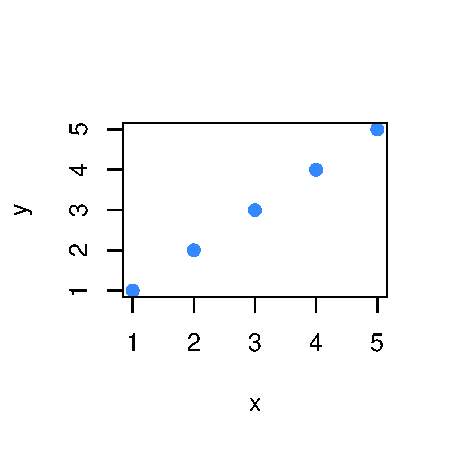
\includegraphics[width=.4\linewidth,height=.4\linewidth]{figure/unnamed-chunk-29-1} 

}



\end{knitrout}

\end{frame}

%------------------------------------------------

\begin{frame}[fragile]
\frametitle{More arguments}

\begin{knitrout}\footnotesize
\definecolor{shadecolor}{rgb}{0.969, 0.969, 0.969}\color{fgcolor}\begin{kframe}
\begin{alltt}
\hlcom{# arguments with and without default values}
\hlstd{myplot} \hlkwb{<-} \hlkwa{function}\hlstd{(}\hlkwc{x}\hlstd{,} \hlkwc{y}\hlstd{,} \hlkwc{col} \hlstd{=} \hlstr{"#3488ff"}\hlstd{,} \hlkwc{pch} \hlstd{=} \hlnum{19}\hlstd{) \{}
  \hlkwd{plot}\hlstd{(x, y,} \hlkwc{col} \hlstd{= col,} \hlkwc{pch} \hlstd{= pch)}
\hlstd{\}}
\end{alltt}
\end{kframe}
\end{knitrout}

\bi
  \item \code{x} and \code{y} have no default values
  \item \code{col} and \code{pch} have default values (but they can be changed)
\ei

\end{frame}

%------------------------------------------------

\begin{frame}[fragile]
\frametitle{More arguments}

\begin{knitrout}\footnotesize
\definecolor{shadecolor}{rgb}{0.969, 0.969, 0.969}\color{fgcolor}\begin{kframe}
\begin{alltt}
\hlcom{# changing default arguments}
\hlkwd{myplot}\hlstd{(}\hlnum{1}\hlopt{:}\hlnum{10}\hlstd{,} \hlnum{10}\hlopt{:}\hlnum{1}\hlstd{,} \hlkwc{col} \hlstd{=} \hlstr{"#994352"}\hlstd{,} \hlkwc{pch} \hlstd{=} \hlnum{18}\hlstd{)}
\end{alltt}
\end{kframe}

{\centering 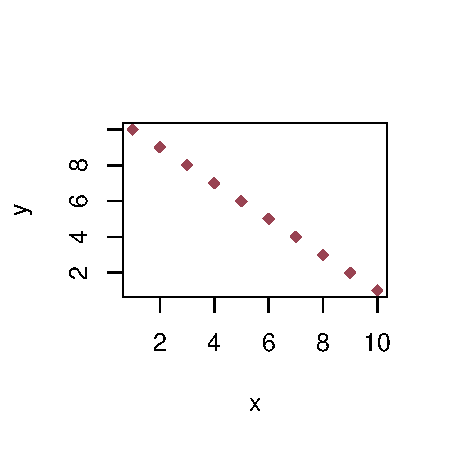
\includegraphics[width=.5\linewidth,height=.5\linewidth]{figure/unnamed-chunk-31-1} 

}



\end{knitrout}

\end{frame}

%------------------------------------------------

\begin{frame}[fragile]
\frametitle{Positional and Named Arguments}

\begin{knitrout}\footnotesize
\definecolor{shadecolor}{rgb}{0.969, 0.969, 0.969}\color{fgcolor}\begin{kframe}
\begin{alltt}
\hlstd{output} \hlkwb{<-} \hlkwd{some_function}\hlstd{(pos1, pos2,} \hlkwc{name1} \hlstd{=} \hlnum{1}\hlstd{,} \hlkwc{name2} \hlstd{=} \hlstr{"yes"}\hlstd{,} \hlkwc{name3} \hlstd{=} \hlkwa{NULL}\hlstd{)}
\end{alltt}
\end{kframe}
\end{knitrout}

\bi
  \item {\hilit \code{pos1}} positional argument
  \item {\hilit \code{pos2}} positional argument
  \item {\hilit \code{name1}} named argument
  \item {\hilit \code{name2}} named argument
  \item {\hilit \code{name3}} named argument
\ei

\end{frame}

%------------------------------------------------

\begin{frame}[fragile]
\frametitle{Argument Matching}

\bi
  \item Arguments with default values are known as \textbf{named} arguments
  \item Arguments with no default values are referred to as \textbf{positional} arguments
  \item Arguments can be matched positionally or by name
\ei

\end{frame}

%------------------------------------------------

\begin{frame}[fragile]
\frametitle{Argument Matching}

\begin{knitrout}\footnotesize
\definecolor{shadecolor}{rgb}{0.969, 0.969, 0.969}\color{fgcolor}\begin{kframe}
\begin{alltt}
\hlstd{values} \hlkwb{<-} \hlkwd{seq}\hlstd{(}\hlopt{-}\hlnum{2}\hlstd{,} \hlnum{1}\hlstd{,} \hlkwc{length.out} \hlstd{=} \hlnum{20}\hlstd{)}

\hlcom{# equivalent calls}
\hlkwd{mean}\hlstd{(values)}
\hlkwd{mean}\hlstd{(}\hlkwc{x} \hlstd{= values)}
\hlkwd{mean}\hlstd{(}\hlkwc{x} \hlstd{= values,} \hlkwc{na.rm} \hlstd{=} \hlnum{FALSE}\hlstd{)}
\hlkwd{mean}\hlstd{(}\hlkwc{na.rm} \hlstd{=} \hlnum{FALSE}\hlstd{,} \hlkwc{x} \hlstd{= values)}
\hlkwd{mean}\hlstd{(}\hlkwc{na.rm} \hlstd{=} \hlnum{FALSE}\hlstd{, values)}
\end{alltt}
\end{kframe}
\end{knitrout}

\end{frame}

%------------------------------------------------

\begin{frame}[fragile]
\frametitle{Partial Matching}

Named arguments can also be partially matched:
\begin{knitrout}\footnotesize
\definecolor{shadecolor}{rgb}{0.969, 0.969, 0.969}\color{fgcolor}\begin{kframe}
\begin{alltt}
\hlcom{# equivalent calls}
\hlkwd{seq}\hlstd{(}\hlkwc{from} \hlstd{=} \hlnum{1}\hlstd{,} \hlkwc{to} \hlstd{=} \hlnum{2}\hlstd{,} \hlkwc{length.out} \hlstd{=} \hlnum{5}\hlstd{)}
\hlkwd{seq}\hlstd{(}\hlkwc{from} \hlstd{=} \hlnum{1}\hlstd{,} \hlkwc{to} \hlstd{=} \hlnum{2}\hlstd{,} \hlkwc{length} \hlstd{=} \hlnum{5}\hlstd{)}
\hlkwd{seq}\hlstd{(}\hlkwc{from} \hlstd{=} \hlnum{1}\hlstd{,} \hlkwc{to} \hlstd{=} \hlnum{2}\hlstd{,} \hlkwc{len} \hlstd{=} \hlnum{5}\hlstd{)}
\end{alltt}
\end{kframe}
\end{knitrout}

\code{length.out} is partially matched with \code{length} and \code{len}

\end{frame}

%------------------------------------------------

\begin{frame}[fragile]
\frametitle{Matching Order}

Order of argument matching operations:
\bbi
  \item Check for exact match for a named argument
  \item Check for a partial match
  \item Check for a positional match
\ei

\end{frame}

%------------------------------------------------

\begin{frame}[fragile]
\frametitle{Example}

Write a function that checks if a number is positive (output \code{TRUE}) or negative (output \code{FALSE})
\pause
\begin{knitrout}\footnotesize
\definecolor{shadecolor}{rgb}{0.969, 0.969, 0.969}\color{fgcolor}\begin{kframe}
\begin{alltt}
\hlstd{is_positive} \hlkwb{<-} \hlkwa{function}\hlstd{(}\hlkwc{x}\hlstd{) \{}
  \hlkwa{if} \hlstd{(x} \hlopt{>} \hlnum{0}\hlstd{)} \hlnum{TRUE} \hlkwa{else} \hlnum{FALSE}
\hlstd{\}}

\hlkwd{is_positive}\hlstd{(}\hlnum{2}\hlstd{)}
\end{alltt}
\begin{verbatim}
## [1] TRUE
\end{verbatim}
\begin{alltt}
\hlkwd{is_positive}\hlstd{(}\hlopt{-}\hlnum{1}\hlstd{)}
\end{alltt}
\begin{verbatim}
## [1] FALSE
\end{verbatim}
\end{kframe}
\end{knitrout}

\end{frame}

%------------------------------------------------

\begin{frame}[fragile]
\frametitle{Example}

Write a function that checks if a number is positive (output \code{TRUE}) or negative (output \code{FALSE})

\begin{knitrout}\footnotesize
\definecolor{shadecolor}{rgb}{0.969, 0.969, 0.969}\color{fgcolor}\begin{kframe}
\begin{alltt}
\hlcom{# a simpler way}
\hlstd{is_positive} \hlkwb{<-} \hlkwa{function}\hlstd{(}\hlkwc{x}\hlstd{) \{}
  \hlstd{x} \hlopt{>} \hlnum{0}
\hlstd{\}}
\end{alltt}
\end{kframe}
\end{knitrout}

\end{frame}

%------------------------------------------------

\begin{frame}[fragile]
\frametitle{Example}

Write a function that checks if a number is positive (output \code{TRUE}) or negative (output \code{FALSE})

\begin{knitrout}\footnotesize
\definecolor{shadecolor}{rgb}{0.969, 0.969, 0.969}\color{fgcolor}\begin{kframe}
\begin{alltt}
\hlcom{# no need to do this}
\hlstd{is_positive} \hlkwb{<-} \hlkwa{function}\hlstd{(}\hlkwc{x}\hlstd{) \{}
  \hlkwa{if} \hlstd{(x} \hlopt{>} \hlnum{0}\hlstd{)} \hlkwd{print}\hlstd{(}\hlstr{'TRUE'}\hlstd{)} \hlkwa{else} \hlkwd{print}\hlstd{(}\hlstr{'FALSE'}\hlstd{)}
\hlstd{\}}
\end{alltt}
\end{kframe}
\end{knitrout}

{\lolit Remember that every function has a value: the last statement that is evaluated (or an output from \code{return()})}

\end{frame}

%------------------------------------------------

\begin{frame}[fragile]
\frametitle{Example}

What happens in these cases?
\begin{knitrout}\footnotesize
\definecolor{shadecolor}{rgb}{0.969, 0.969, 0.969}\color{fgcolor}\begin{kframe}
\begin{alltt}
\hlkwd{is_positive}\hlstd{(}\hlnum{0}\hlstd{)}

\hlkwd{is_positive}\hlstd{(}\hlnum{NA}\hlstd{)}

\hlkwd{is_positive}\hlstd{(}\hlnum{TRUE}\hlstd{)}

\hlkwd{is_positive}\hlstd{(}\hlstr{"positive"}\hlstd{)}

\hlkwd{is_positive}\hlstd{(}\hlnum{1}\hlopt{:}\hlnum{5}\hlstd{)}
\end{alltt}
\end{kframe}
\end{knitrout}

\end{frame}

%------------------------------------------------

\begin{frame}[fragile]
\frametitle{Using arguments for other functions}

Theere are various functions that include the argument {\hilit \code{na.rm}} to indicate if missing values should be removed. One of them is \code{mean()}:
\begin{knitrout}\footnotesize
\definecolor{shadecolor}{rgb}{0.969, 0.969, 0.969}\color{fgcolor}\begin{kframe}
\begin{alltt}
\hlcom{# deafult na.rm = FALSE}
\hlkwd{mean}\hlstd{(}\hlkwd{c}\hlstd{(}\hlnum{1}\hlstd{,} \hlnum{2}\hlstd{,} \hlnum{3}\hlstd{,} \hlnum{NA}\hlstd{,} \hlnum{5}\hlstd{))}
\end{alltt}
\begin{verbatim}
## [1] NA
\end{verbatim}
\begin{alltt}
\hlcom{# deafult na.rm = TRUE}
\hlkwd{mean}\hlstd{(}\hlkwd{c}\hlstd{(}\hlnum{1}\hlstd{,} \hlnum{2}\hlstd{,} \hlnum{3}\hlstd{,} \hlnum{NA}\hlstd{,} \hlnum{5}\hlstd{),} \hlkwc{na.rm} \hlstd{=} \hlnum{TRUE}\hlstd{)}
\end{alltt}
\begin{verbatim}
## [1] 2.75
\end{verbatim}
\end{kframe}
\end{knitrout}

\end{frame}

%------------------------------------------------

\begin{frame}[fragile]
\frametitle{Using arguments for other functions}

If we create a function that uses other functions containing \code{na.rm}, it is wise to include that argument:
\begin{knitrout}\footnotesize
\definecolor{shadecolor}{rgb}{0.969, 0.969, 0.969}\color{fgcolor}\begin{kframe}
\begin{alltt}
\hlstd{meansd} \hlkwb{<-} \hlkwa{function}\hlstd{(}\hlkwc{x}\hlstd{,} \hlkwc{na.rm} \hlstd{=} \hlnum{FALSE}\hlstd{) \{}
  \hlkwd{c}\hlstd{(}\hlkwc{mean} \hlstd{=} \hlkwd{mean}\hlstd{(x,} \hlkwc{na.rm} \hlstd{= na.rm),}
    \hlkwc{sd} \hlstd{=} \hlkwd{sd}\hlstd{(x,} \hlkwc{na.rm} \hlstd{= na.rm))}
\hlstd{\}}

\hlkwd{meansd}\hlstd{(}\hlkwd{c}\hlstd{(}\hlnum{1}\hlstd{,} \hlnum{2}\hlstd{,} \hlnum{3}\hlstd{,} \hlnum{NA}\hlstd{,} \hlnum{5}\hlstd{),} \hlkwc{na.rm} \hlstd{=} \hlnum{TRUE}\hlstd{)}
\end{alltt}
\begin{verbatim}
##     mean       sd 
## 2.750000 1.707825
\end{verbatim}
\end{kframe}
\end{knitrout}

\end{frame}

%------------------------------------------------

\begin{frame}[fragile]
\frametitle{Dots argument}

If you check functions like \code{c()}, \code{paste()}, \code{plot()}, you'll notice the use of a special argument: {\hilit \code{\dots}}

\bi
  \item it matches zero, one or more actual arguments
  \item it allows us to pass arguments to other functions inside the function
  \item \code{\dots} allows us to ``cascade'' arguments to other functions without inluding them in the definition
\ei

\end{frame}

%------------------------------------------------

\begin{frame}[fragile]
\frametitle{Dots argument}

Using \code{\dots}
\begin{knitrout}\footnotesize
\definecolor{shadecolor}{rgb}{0.969, 0.969, 0.969}\color{fgcolor}\begin{kframe}
\begin{alltt}
\hlstd{fplot} \hlkwb{<-} \hlkwa{function}\hlstd{(}\hlkwc{y}\hlstd{,} \hlkwc{...}\hlstd{) \{}
  \hlstd{x} \hlkwb{<-} \hlnum{1}\hlopt{:}\hlkwd{length}\hlstd{(y)}
  \hlkwd{plot}\hlstd{(x, y,} \hlkwc{type} \hlstd{=} \hlstr{'n'}\hlstd{,} \hlkwc{ylim} \hlstd{=} \hlkwd{c}\hlstd{(}\hlnum{0}\hlstd{,} \hlnum{1}\hlstd{), ...)}
  \hlkwd{points}\hlstd{(x, y,} \hlkwc{col} \hlstd{=} \hlstr{"#93a8f2"}\hlstd{,} \hlkwc{pch} \hlstd{=} \hlnum{19}\hlstd{)}
  \hlkwd{lines}\hlstd{(x, y,} \hlkwc{col} \hlstd{=} \hlstr{"#dd93f2"}\hlstd{,} \hlkwc{lwd} \hlstd{=} \hlnum{3}\hlstd{)}
\hlstd{\}}

\hlkwd{fplot}\hlstd{(}\hlkwd{runif}\hlstd{(}\hlnum{10}\hlstd{),} \hlkwc{bty} \hlstd{=} \hlstr{'n'}\hlstd{)}
\hlkwd{fplot}\hlstd{(}\hlkwd{runif}\hlstd{(}\hlnum{10}\hlstd{),} \hlkwc{bty} \hlstd{=} \hlstr{'n'}\hlstd{,} \hlkwc{main} \hlstd{=} \hlstr{"some title"}\hlstd{)}
\hlkwd{fplot}\hlstd{(}\hlkwd{runif}\hlstd{(}\hlnum{10}\hlstd{),} \hlkwc{bty} \hlstd{=} \hlstr{'n'}\hlstd{,} \hlkwc{xlab} \hlstd{=} \hlstr{''}\hlstd{)}
\end{alltt}
\end{kframe}
\end{knitrout}

\end{frame}

%------------------------------------------------

\end{document}
